\documentclass[a4paper,12pt]{report}

\usepackage{cmap}
\usepackage[T2A]{fontenc}
\usepackage[utf8]{inputenc}
\usepackage[russian]{babel}
\usepackage{amsmath,amsfonts,amssymb}
\usepackage{graphicx}
\usepackage{sidecap}
\usepackage{wrapfig}


\begin{document} 

\begin{titlepage} 

\begin{center} 

\large Федеральное государственное автономное образовательное учреждение высшего образования «Санкт-Петербургский государственный электротехнический университет «ЛЭТИ» им. В.И. Ульянова (Ленина)»
	
кафедра теоретических основ электротехники\\[5cm] 

\huge ОТЧЕТ\\ по лабораторной работе № 2\\[0.5cm] 
\large <<ИССЛЕДОВАНИЕ ЛИНЕЙНЫХ РЕЗИСТИВНЫХ ЦЕПЕЙ>>\\[3.7cm]

\begin{minipage}{1\textwidth} 
    \begin{flushleft} 
        \emph{Авторы:} Стукен В.А. , Зиновьев М.Д\\
        \emph{Группа:} 2307\\
        \emph{Факультет:} ФКТИ\\
        \emph{Преподаватель:} Зубарев А.В
    \end{flushleft} 
\end{minipage} 

\vfill 

Санкт-Петербург, 2024\\
{\large \LaTeX} 

\end{center} 

\thispagestyle{empty} 
\end{titlepage} 

\section*{Экспериментальные исследования}

\begin{flushleft}
    \item\subsection*{Опыт №1 Исследование цепи при питании ее от двух источников}
    \item \begin{figure}[h!]
        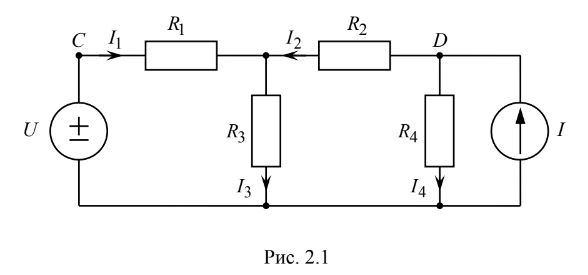
\includegraphics[width=1.1\textwidth]{scheme_1.png}
        \label{ris:image1}
    \end{figure}
    
    \resizebox{15cm}{!}{ 
        \begin{tabular}{|l|l|l|l|l|l|l|l|l|l|}
                \hline
                 $U, V$ & $ U_1$ & $U_2$ & $U_3$ & $U_4$ & $I, mA$ & $I_1$ & $I_2$ & $I_3$ & $I_4$   \\
                \hline
                2 & 0.37 & 0.44 & 1.62 & 2.06 & 1.03 & 0.26 & 0.29 & 0.56 & 0.72 \\
				\hline
        \end{tabular}
    }
    \[  U=U_1+U_3=0,37+1,62=1,99      \]
    \[  I=I_2+I_4=0,29+0,72=1,01   \] 
    \[  U_4=U_2+U_3=0,44+1,62=2,06 \] 
    \[  I_3=I_1+I_2=0,26+0,29=0,55 \]
    \newpage

	\item\subsection*{Опыт №2 Определение тока в цепи методом наложения}
	\item \item \begin{figure}[h!]
        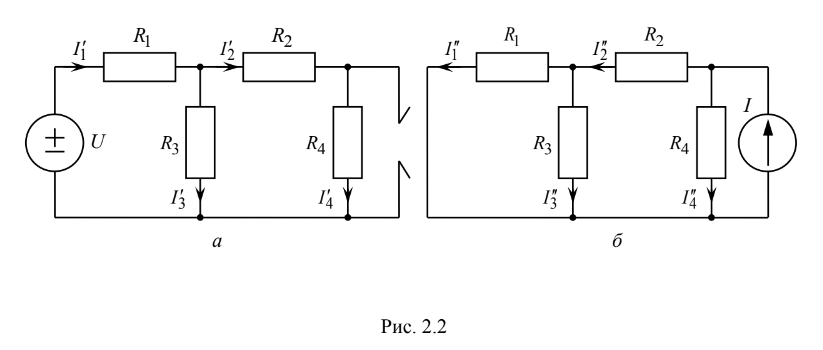
\includegraphics[width=1.1\textwidth]{scheme_2.png}
        \label{ris:image2}
    \end{figure}
    \resizebox{10cm}{!}{ 
        \begin{tabular}{|l|l|l|l|l|}
                \hline
                 $  $ & $I_1, mA$ & $I_2$ & $I_3$ & $I_4$ \\
                \hline
                U & 0.61 & 0.24 & 0.36 & 0.25 \\
				\hline
				I & 0.36 & 0.55 & 0.18 & 0.48 \\
				\hline
				I,U & 0.25 & 0.31 & 0.54 & 0.73 \\
				\hline
        \end{tabular}
    }
    \[I_1=I_1^a-I_1^b     I_2=I_2^b-I_2^a    I_3=I_3^a+I_3^b     I_4=I_4^a+I_4^b\]

    Полученные значения сравнимы с теми, которые были получены при работе обоих источников.
    
    \newpage
	\item\subsection*{Опыт №3 Определение тока в ветви с сопротивлением R3 методом эквивалентного источника напряжения}
	\item \item \begin{figure}[h!]
        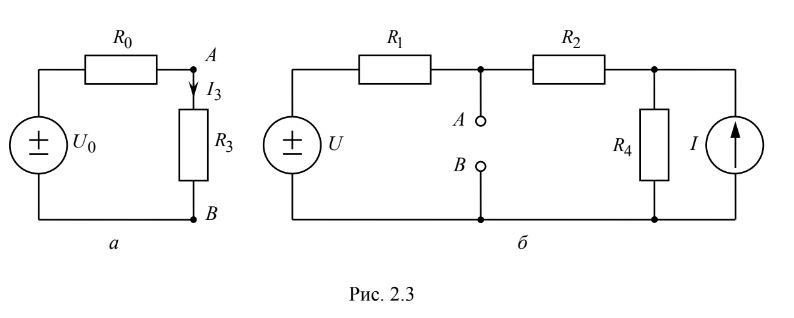
\includegraphics[width=1.1\textwidth]{scheme_3.png}
        \label{ris:image3}
    \end{figure}

    \subsection*{Запишем уравнения МКТ:}
    \[\begin{cases}
        i_1^k = I = 0.00103 &
      \\
        (R1+R2+R4)\cdot i_2^k - R_4i_1^k = -U &
      \end{cases}
    \]
    \[\begin{cases}
        i_1^k = 0.00103 &
      \\
        i_2^k = 0.000181 &
      \end{cases}\]
    \[ i_{R1} = -i_2^k = -0.000181 \]
    
    \[ U = U_{xx} + U_{R1} \]
    \[ 2 = U_{xx} - 0.000181 \cdot 1500 \]
    \[ U_{xx} = 2.27 \]
    
    \newpage
    \subsection*{Найдем Rэкв}
    \begin{figure}[h!]
        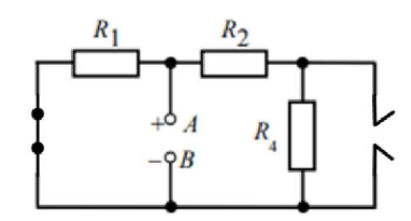
\includegraphics[width=1.0\textwidth]{scheme_5.png}
        \label{ris:image5}
    \end{figure}

    \[ R_{ekv} = \frac{R_1(R_2 + R_4)}{R_1+R_2+R_4} = 1.125 \, k\Omega  \]

    \subsection*{Найдем ток $i_{R3}$}
    \[ i_{R3} = \frac{U_{xx}}{R_{ekv} + R_3} = \frac{2.27}{1125 + 3000} = 0.55 \, mA \]

	\newpage
	\item\subsection*{Опыт №4 Экспериментальная проверка принципа взаимности}
	\item \item \begin{figure}[h!]
        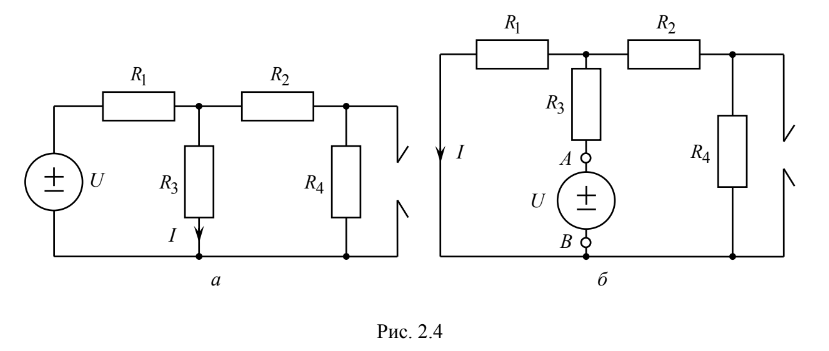
\includegraphics[width=1.1\textwidth]{scheme_4.png}
        \label{ris:image4}
    \end{figure}
    По МКТ: 
    \[\begin{cases}
        4.5i_1^k + 3i_2^k = 2 &
      \\
        3*i_1^k + 7.5i_2^k = 0 &
    \end{cases}\]
    \[\begin{cases}
    i_1^k = 0.6 &
      \\
    i_2^k  = -0.24 &
    \end{cases}\]
     
Токи в цепях а $I_3 = 0.36 \, mA $ и б $I_3=0,36\, mA$ равны, это подтверждает принцип взаимности.

\end{flushleft}
\newpage

\section*{Ответы на вопросы}

\begin{itemize}
    \item Вопрос №1: \textbf{Каковы результаты контроля данных в 2.2.1?}
    \par Проверили полученные значения по законам Кирхгофа, они сошлись с учетом измерительной погрешности.
    \item Вопрос №2: \textbf{Изменятся ли токи ветвей, если одновременно изменить полярность напряжения ИН и направление тока ИТ на противоположные?}
    \par Изменится знак токов на противоположные, модули останутся такими же.
    \item Вопрос №3: \textbf{Чему равно напряжение между узлами «C» и «D» цепи?}
    \[ U_{CD} = U_1 - U_2 = 0.37 - 0.44 = -0.07 \]
    \item Вопрос №4: \textbf{Как изменить напряжение ИН, чтобы ток $I_1$ стал равен нулю?}
    \par 	Из метода наложения выполняется $I_1=I_1^a-I_1^b$, тогда $I_1^a=I_1^b=0,36$
    $U= I_{need}/I_{real} \cdot U = 0,36/0,61 \cdot 2=1,23$
    
    \item Вопрос №5: \textbf{Почему рис. 2.4, б при $U = U_0$
    реализует схему метода эквивалентного источника напряжения \\(рис. 2.3, а)?}
    \par Так как $R_0 = \frac{R_1(R_2+R_4)}{R_1+R_2+R_4}$, то есть схемы 2.4б и 2.3а одинаковые.
    \item Вопрос №6: \textbf{Чему будет равен ток $I_1$, если ИН поместить в
    ветвь 4, а ИТ отключить?}
    \par Используя принцип взаимности, $I_1 = 0.36$
    \item Вопрос №7: \textbf{Как проконтролировать результаты эксперимен-
    тов в 2.2.2, 2.2.3 и 2.2.4?}
    \par Сравнивая полученные в первом пункте значения каждого элемента.
    
\end{itemize}
\newpage
\section*{Вывод}
В данной экспериментальной работе мы провели анализ резистивной цепи, состоящей из источников постоянного тока и напряжения. Мы измерили токи и напряжения в цепи и проверили их согласованность с уравнениями Киргофа. При расчетах применили различные методики, включая метод наложения, использование эквивалентного источника и принцип взаимности. Интересное наблюдение: если единственный источник напряжения действует в одной ветви линейной электрической цепи и вызывает ток в другой ветви, то после его перемещения во вторую ветвь он вызовет в первой ветви такой же ток.
\newpage





\end{document}
